\chapter{Design}
The following chapter shall discuss the planning and design choices of the system. 



\newpage
\section{TODO Sequence Diagram}

\newpage
\section{Interface}

\begin{figure}[H]
    \centering
    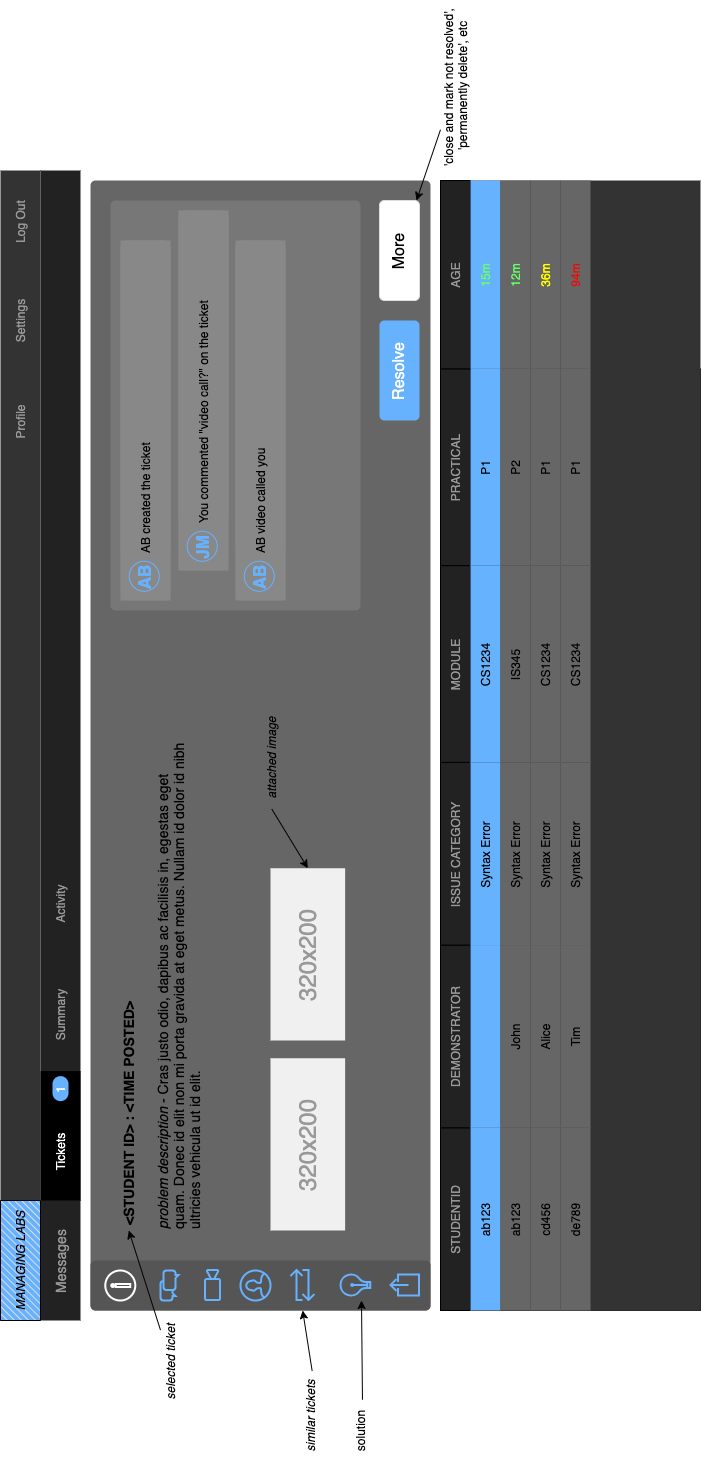
\includegraphics[width=0.6\textwidth]{7design/images/demoTickets.png}
    \caption{Simple design for the demo ticket viewing interface.}
    \label{fig:demoTickets}
\end{figure}

\section{Database}

\subsection{Entities, Attributes and Relationships}
We will now define a representation of the data in terms of entities, attributes and relationships between entities.

\subsubsection{Entities}

We represent the components of the systems as the following entities. 

\FloatBarrier
\begin{table}[H]
\centering
\begin{tabular}{ |l|c| } 
 \hline
 \textbf{Entity Set} & \textbf{Attributes}\\ 
 \hline
  user & \underline{studentId}, name, userType, password, loginStatus\\ 
 \hspace{6pt}user.student & enrolledModules\\ 
 \hspace{6pt}user.demonstrator & demonstratedModules\\
 \hspace{12pt}user.demonstrator.labLead & ledModules\\
 sysAdmin & \underline{username}, password\\ 
 ticket & \underline{ticketId}, category, issueDescription, module,\\
 & practical, attachedFiles, comments, resolutionStatus \\
 lab & \underline{labId}, openTime, closeTime, demonstrators\\
 solution & \underline{solutionId}, category, solutionText, attachedFiles\\
 \hline
\end{tabular}
\caption{Table of entities and associated attributes.}
\end{table}
\FloatBarrier

Primary keys are denoted as \underline{underlined}. Foreign keys are denoted in \textit{italics}.

Note that \textbf{user.student} and \textbf{user.demonstrator} are disjoint specialisations of the entity set \textbf{user} - a user is always a student or demonstrator (or specialisation of demonstrator). \textbf{user.demonstrator.labLead} is a further specialisation of \textbf{user.demonstrator}, not disjoint. 

\subsubsection{Relationships}
We shall now define the relationships between entities and the constraints on them. 

\FloatBarrier
\begin{table}[H]
\centering
\begin{tabular}{ |c|c|c|c| } 
 \hline
 \textbf{Relationship} & \textbf{Entities} & \textbf{Participation} & \textbf{Cardinality}\\ 
 \hline
 $r$ & $e_1$, $e_2$ & total, partial & M-1 \\
 \hline
\end{tabular}
\end{table}
\FloatBarrier 

We denote many as M, one as 1 such that one to many relationship would be denoted 1-M. Note that for a relationship $r$ that is many (in $e_1$) to one (in $e_2$) and has total participation from $e_1$ but partial from $e_2$ then the row in the table is written as above. Participation will be listed in order that entities are written.

\FloatBarrier
\begin{table}[htbp]
\centering
\resizebox{\columnwidth}{!}{\begin{tabular}{ |c|c|c|c|c| } 
 \hline
 \textbf{Relationship} & \textbf{Relationship Attributes} & \textbf{Entity Sets} & \textbf{Participation} & \textbf{Cardinality}\\ 
 \hline
 creates & creation\_timestamp & user.student, ticket & partial, total & 1-M \\
 manages & demAssigned\_timestamp & user.demonstrator, ticket & partial, partial & 1-M\\
 writes & demSolved\_timestamp & user.demonstrator, solution & partial, total & M-M\\
 leads & & user.demonstrator.labLead, lab & partial, total & 1-M \\
 \hline
\end{tabular}}
\caption{Table showing entities, relationships between, relationship attributes, participation and cardinality.}
\end{table}
\FloatBarrier